%%%%%%%%%%%%%%%%%%%%%%%%%%%%%%%%%%%%%%%%%
% Beamer Presentation
% LaTeX Template
% Version 1.0 (10/11/12)
%
% This template has been downloaded from:
% http://www.LaTeXTemplates.com
%
% License:
% CC BY-NC-SA 3.0 (http://creativecommons.org/licenses/by-nc-sa/3.0/)
%
%%%%%%%%%%%%%%%%%%%%%%%%%%%%%%%%%%%%%%%%%

%----------------------------------------------------------------------------------------
%	PACKAGES AND THEMES
%----------------------------------------------------------------------------------------

\documentclass{beamer}

\mode<presentation> {

% The Beamer class comes with a number of default slide themes
% which change the colors and layouts of slides. Below this is a list
% of all the themes, uncomment each in turn to see what they look like.

% \usetheme{default}
%\usetheme{AnnArbor}
%\usetheme{Antibes}
%\usetheme{Bergen}
% \usetheme{Berkeley}
%\usetheme{Berlin}
%\usetheme{Boadilla}
%\usetheme{CambridgeUS}
%\usetheme{Copenhagen}
%\usetheme{Darmstadt}
%\usetheme{Dresden}
%\usetheme{Frankfurt}
%\usetheme{Goettingen}
%\usetheme{Hannover}
%\usetheme{Ilmenau}
%\usetheme{JuanLesPins}
%\usetheme{Luebeck}
%\usetheme{Madrid}
%\usetheme{Malmoe}
%\usetheme{Marburg}
%\usetheme{Montpellier}
%\usetheme{PaloAlto}
%\usetheme{Pittsburgh}
%\usetheme{Rochester}
%\usetheme{Singapore}
%\usetheme{Szeged}
%\usetheme{Warsaw}

% As well as themes, the Beamer class has a number of color themes
% for any slide theme. Uncomment each of these in turn to see how it
% changes the colors of your current slide theme.

%\usecolortheme{albatross}
%\usecolortheme{beaver}
%\usecolortheme{beetle}
%\usecolortheme{crane}
%\usecolortheme{dolphin}
%\usecolortheme{dove}
%\usecolortheme{fly}
%\usecolortheme{lily}
%\usecolortheme{orchid}
%\usecolortheme{rose}
%\usecolortheme{seagull}
\usecolortheme{seahorse}
%\usecolortheme{whale}
%\usecolortheme{wolverine}

%\setbeamertemplate{footline} % To remove the footer line in all slides uncomment this line
%\setbeamertemplate{footline}[page number] % To replace the footer
%line in all slides with a simple slide count uncomment this line

%\setbeamertemplate{navigation symbols}{} % To remove the navigation
%symbols from the bottom of all slides uncomment this line
}

\usepackage{graphicx} % Allows including images
\usepackage{booktabs} % Allows the use of \toprule, \midrule and \bottomrule
                      % in tables

\DeclareGraphicsExtensions{.pdf,.png,.jpg}
\usepackage{amssymb,amsmath,amsthm,amsfonts}
\usepackage{mathrsfs}
\usepackage{dsfont}
\usepackage{enumerate}

%\newtheorem{mdef}{Definition}
%\newtheorem{theorem}{Theorem}
\newcommand{\eqsplit}[2]{
  \begin{equation}\label{#2}
    \begin{split}
      #1
    \end{split}
  \end{equation}}
\newcommand{\eqnsplit}[1]{
  \begin{eqnarray*}
    #1
  \end{eqnarray*}}
\newcommand{\tran}[1]{
  \tilde{#1}
}
\newcommand{\td}[2]{
  \frac{d #1}{d #2}
}
\newcommand{\pd}[2]{
  \frac{\partial #1}{\partial #2}
}
\newcommand{\ppd}[2]{
  \frac{\partial^2 #1}{\partial #2^2}
}
\newcommand{\pdd}[3]{
  \frac{\partial^2 #1}{\partial #2 \partial #3}
}
\newcommand{\otd}[1]{
  \frac{d}{d #1}
}
\newcommand{\opd}[1]{
  \frac{\partial}{\partial #1}
}
\newcommand{\oppd}[1]{
  \frac{\partial^2}{\partial #1^2}
}
\newcommand{\opdd}[2]{
  \frac{\partial^2}{\partial #1 \partial #2}
}
\newcommand{\ket}[1]{
  |#1\rangle
}
\newcommand{\bra}[1]{
  \langle#1|
}
\newcommand{\inn}[1]{
  \langle#1\rangle
}
\newcommand{\mean}[1]{
  \langle#1\rangle
}
\newcommand{\tr}{
  \text{tr}\,
}
\newcommand{\re}{
  \text{Re}\,
}
\newcommand\im{
  \text{Im}\,
}
\newcommand{\var}{
  \text{var}
}
\newcommand{\arcsinh}{
  \sinh^{-1}
}
\newcommand{\arccosh}{
  \cosh^{-1}
}
\newcommand{\erfc}{
  \text{erfc}
}
\newcommand{\E}{
  \mathbb{E}
}
\renewcommand{\P}{
  \mathbb{P}
}
\newcommand{\I}[1]{
  \mathbf{1}_{\{#1\}}
}
\newcommand{\1}[1]{
  \mathds{1}_{\{#1\}}
}
\newcommand{\diag}{
  \text{diag\,}
}
\newcommand{\M}{
  {\text{max}}
}
\newcommand{\m}{
  {\text{min}}
}
\newcommand{\ph}{
  {\text{arg}\,}
}
\newcommand\erf{
  \text{erf}
}
\renewcommand\vec[1]{
  \mathbf{#1}
}
\newcommand\mtx[1]{
  \mathbf{#1}
}
\newcommand\ed{
  \,{\buildrel d \over =}\,
}




%----------------------------------------------------------------------------------------
%	TITLE PAGE
%----------------------------------------------------------------------------------------

\title{Some Results on GARCH processes and their Applications to Financial Times Series}
% The short title appears at the bottom of
% every slide, the full title is only
% on the title page

\author{Xie Xiaolei} % Your name
\institute[UCPH] % Your institution as it will appear on the bottom of every slide, may be shorthand to save space
{
Copenhagen University  \\ % Your institution for the title page
\medskip
\textit{xie@math.ku.dk} % Your email address
}
\date{\today} % Date, can be changed to a custom date

\begin{document}

\begin{frame}
\titlepage % Print the title page as the first slide
\end{frame}

% \begin{frame}
% \frametitle{Overview}
% \tableofcontents
% \end{frame}

%----------------------------------------------------------------------------------------
%	PRESENTATION SLIDES
%----------------------------------------------------------------------------------------
% \section{Simple dependence models}
%------------------------------------------------
\section{Some Empirical Results}
\subsection{FX Series}
\begin{frame}
  \begin{figure}[htb!]
    \centering
    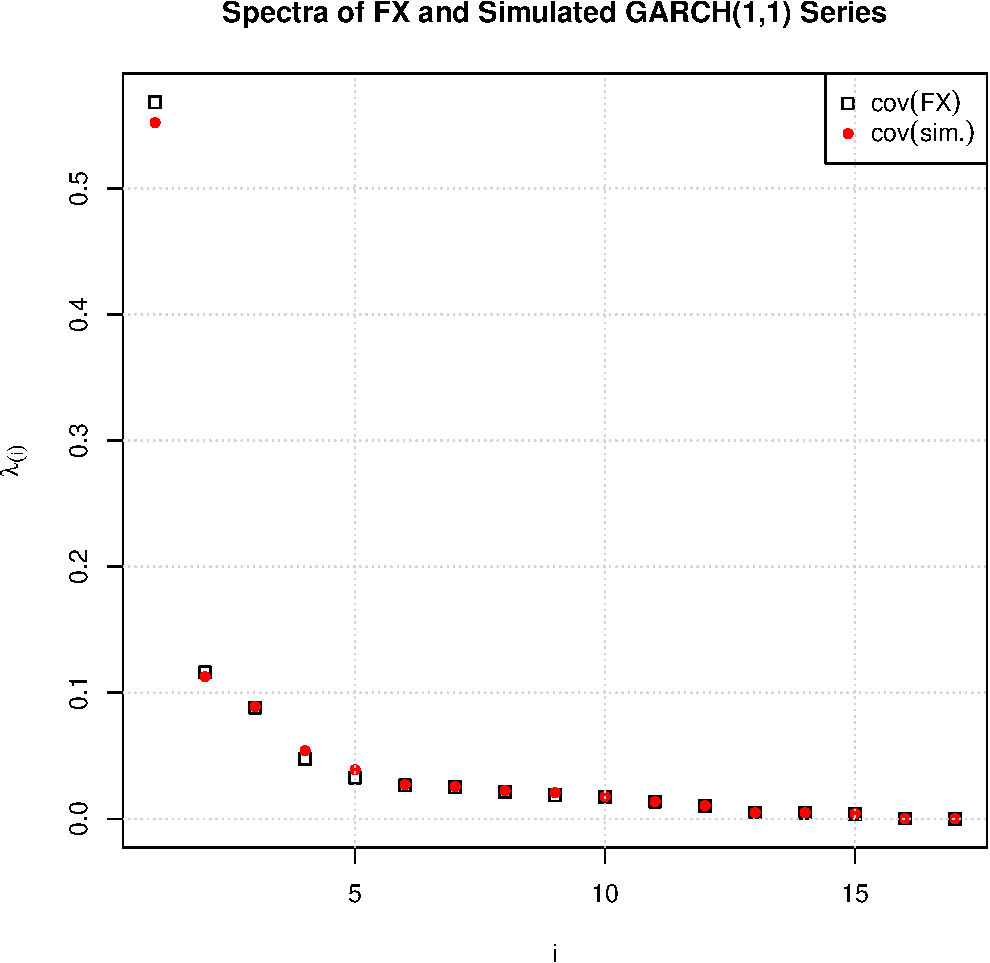
\includegraphics[scale=0.35]{FX_eigenvalues.pdf}
    \caption{\scriptsize Eigenvalues of real FX series and Simulated GARCH(1,1) series}
  \end{figure}
\end{frame}

\begin{frame}
  \begin{figure}[htb!]
    \centering
    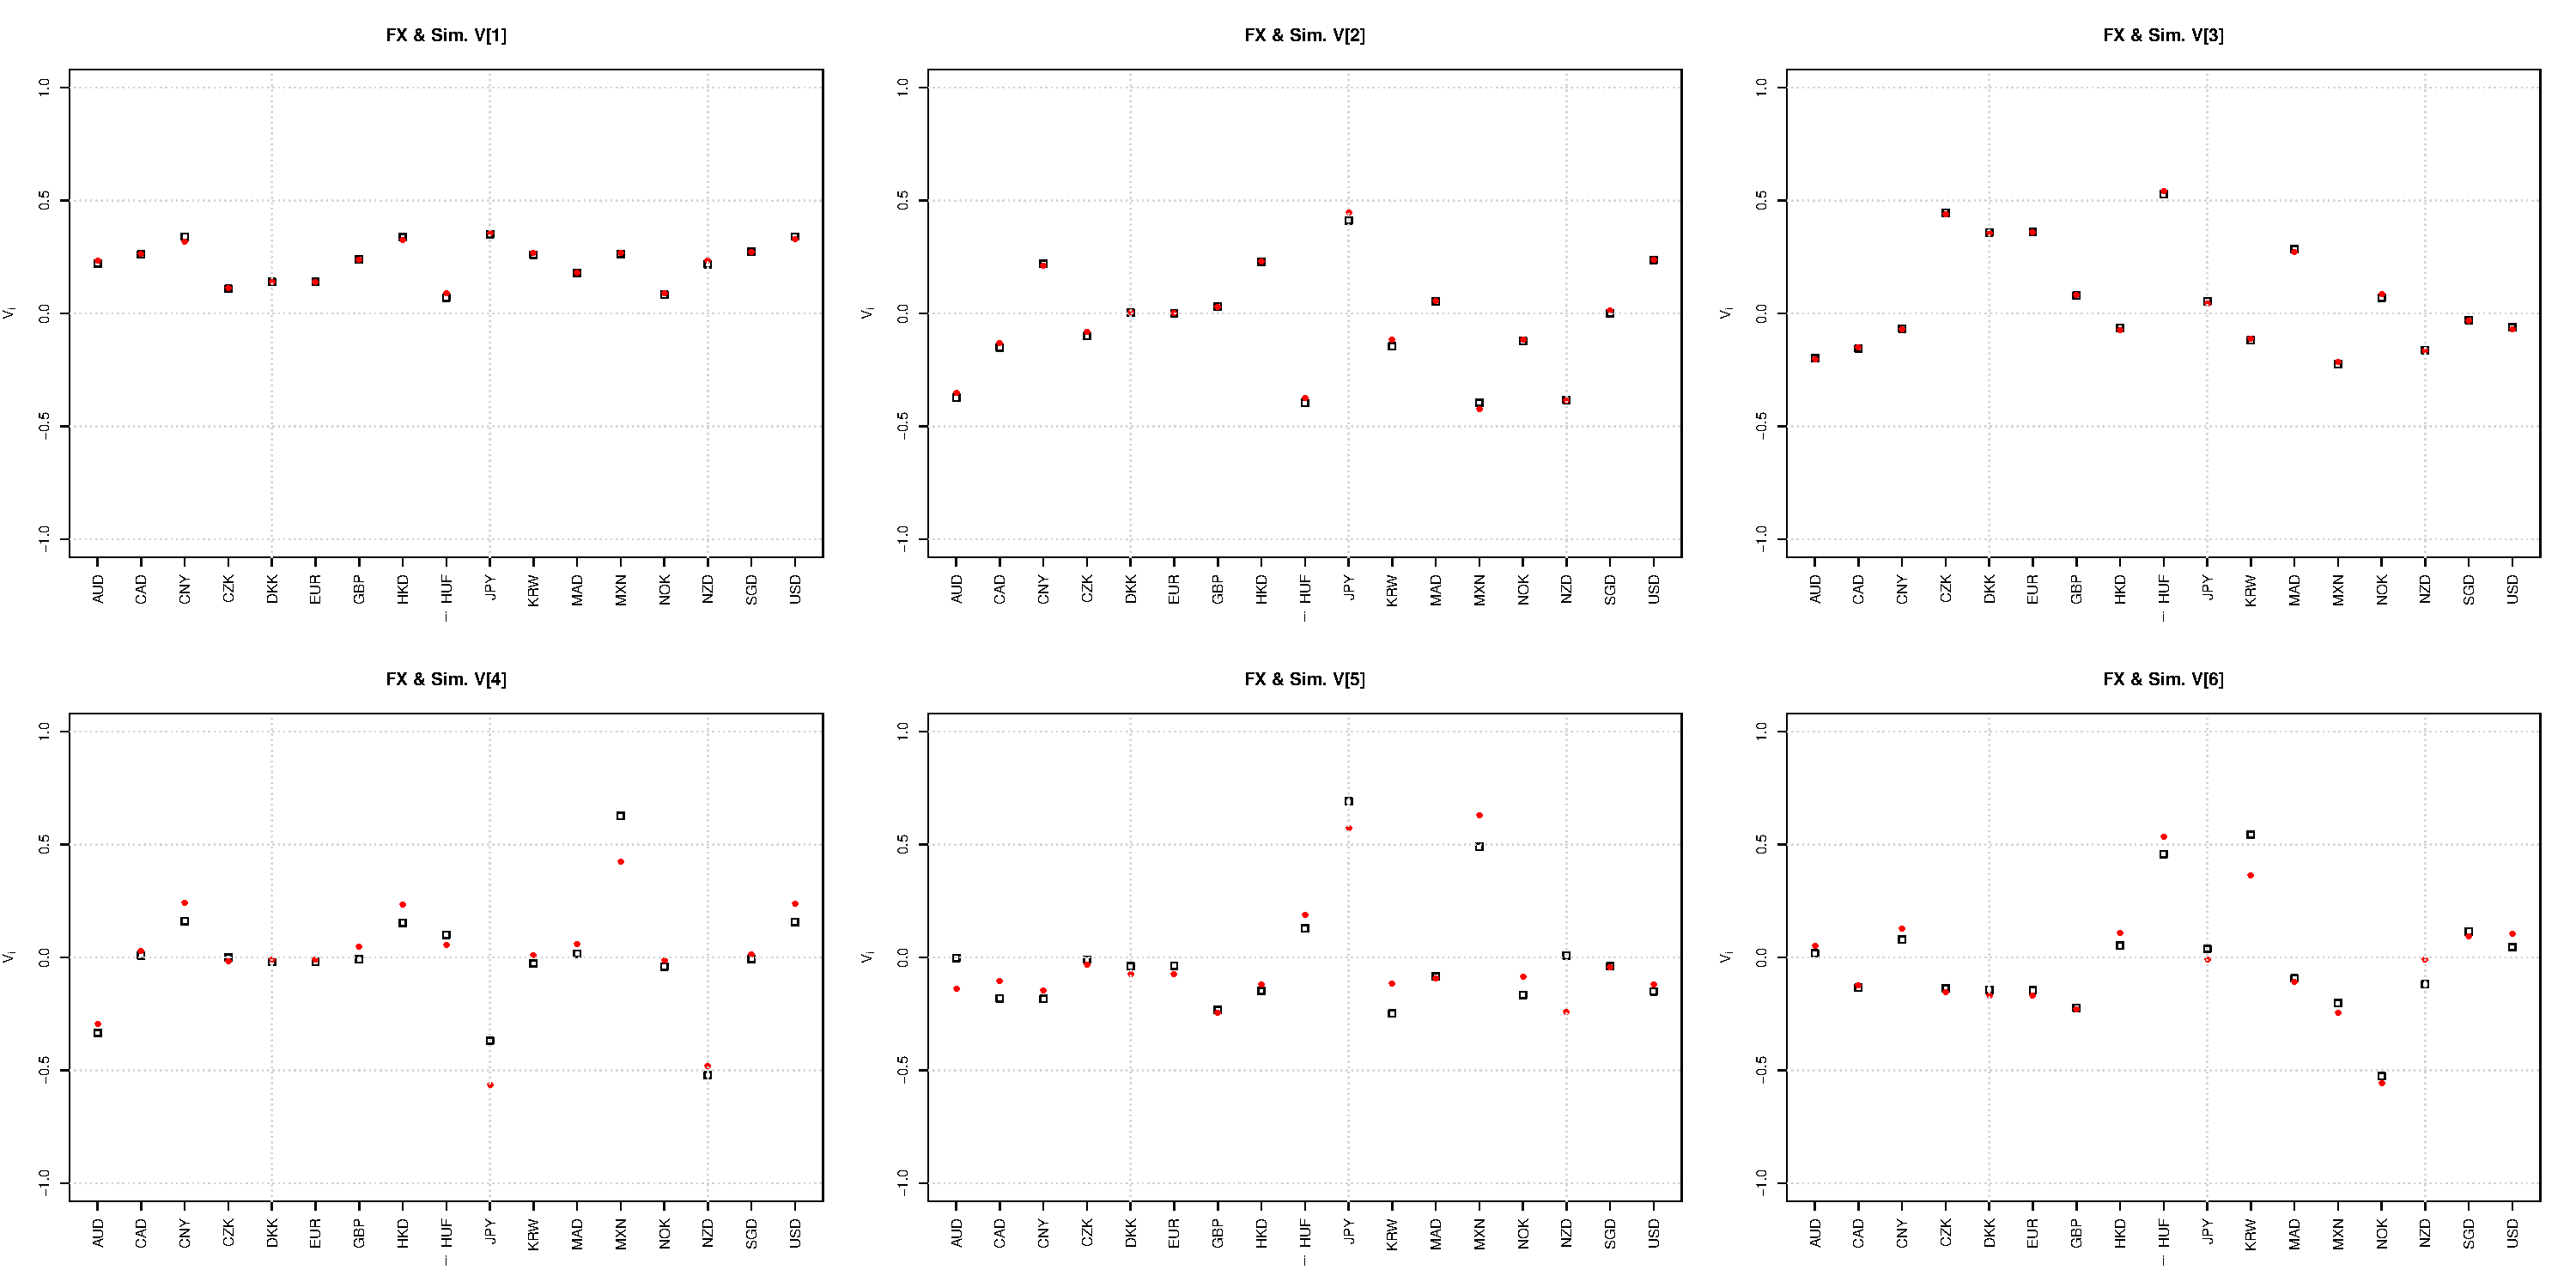
\includegraphics[scale=0.2]{FX_eigenvectors.pdf}
    \caption{\scriptsize Eigenvectors of real FX series and Simulated GARCH(1,1) series}
  \end{figure}
\end{frame}

\begin{frame}
  The FX series are modeled with:
  \begin{eqnarray*}
    X_{i, t} &=& \sigma_{i, t} Z_{i, t} \\
    \sigma_{i, t}^2 &=& \alpha_{i} X_{i, t}^2 + \beta_{i} \sigma_{i, t-1}^2 + \omega_i \\
    (Z_{1, t}, ..., Z_{p, t}) &\sim& N(0, \Sigma) \\
    \var(Z_{i,t}) &=& 1
  \end{eqnarray*}
\end{frame}

\begin{frame}
  \frametitle{Gaussian Series with the same Covariance Matrix as the
    Observations}
  \begin{figure}[htb!]
    \centering
    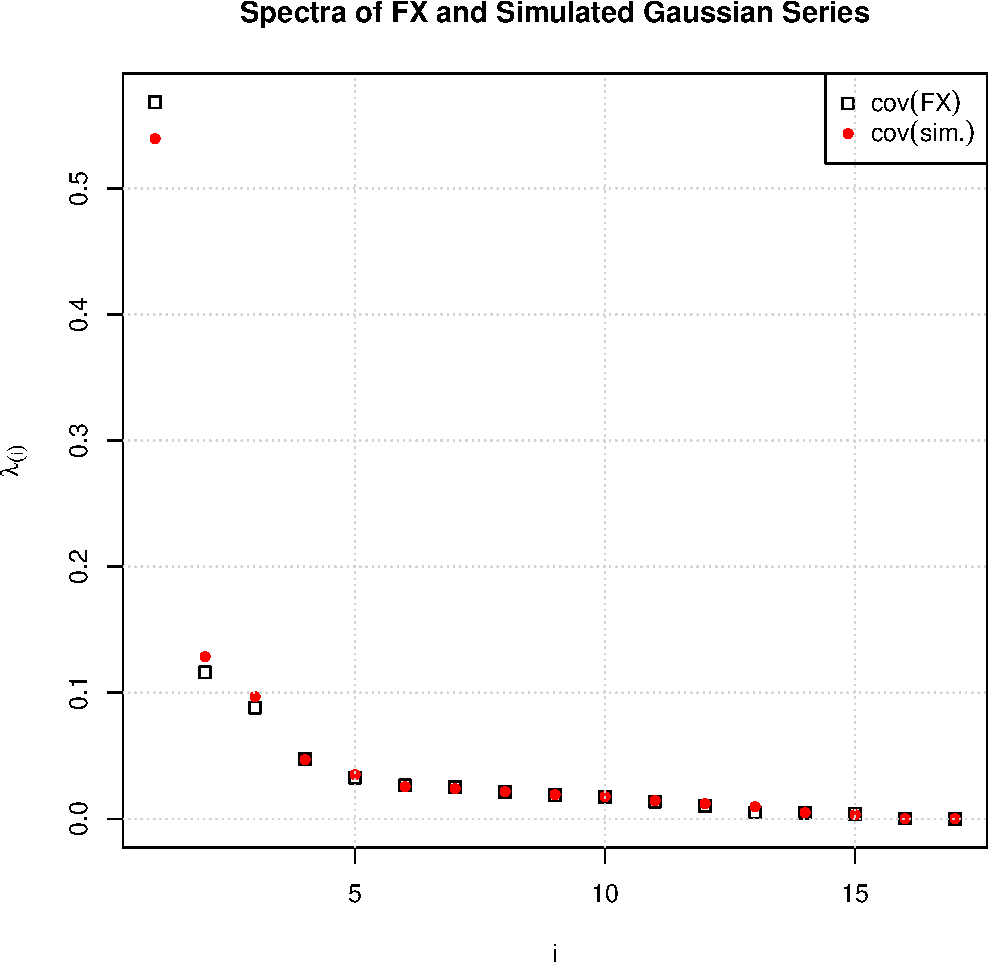
\includegraphics[scale=0.35]{Gaussian_eigenvalues.pdf}
    \caption{\scriptsize Eigenvalues of real FX series and Simulated Gaussian series}
  \end{figure}
\end{frame}

\begin{frame}
  \frametitle{Gaussian Series with the same Covariance Matrix as the Observations}
  \begin{figure}[htb!]
    \centering
    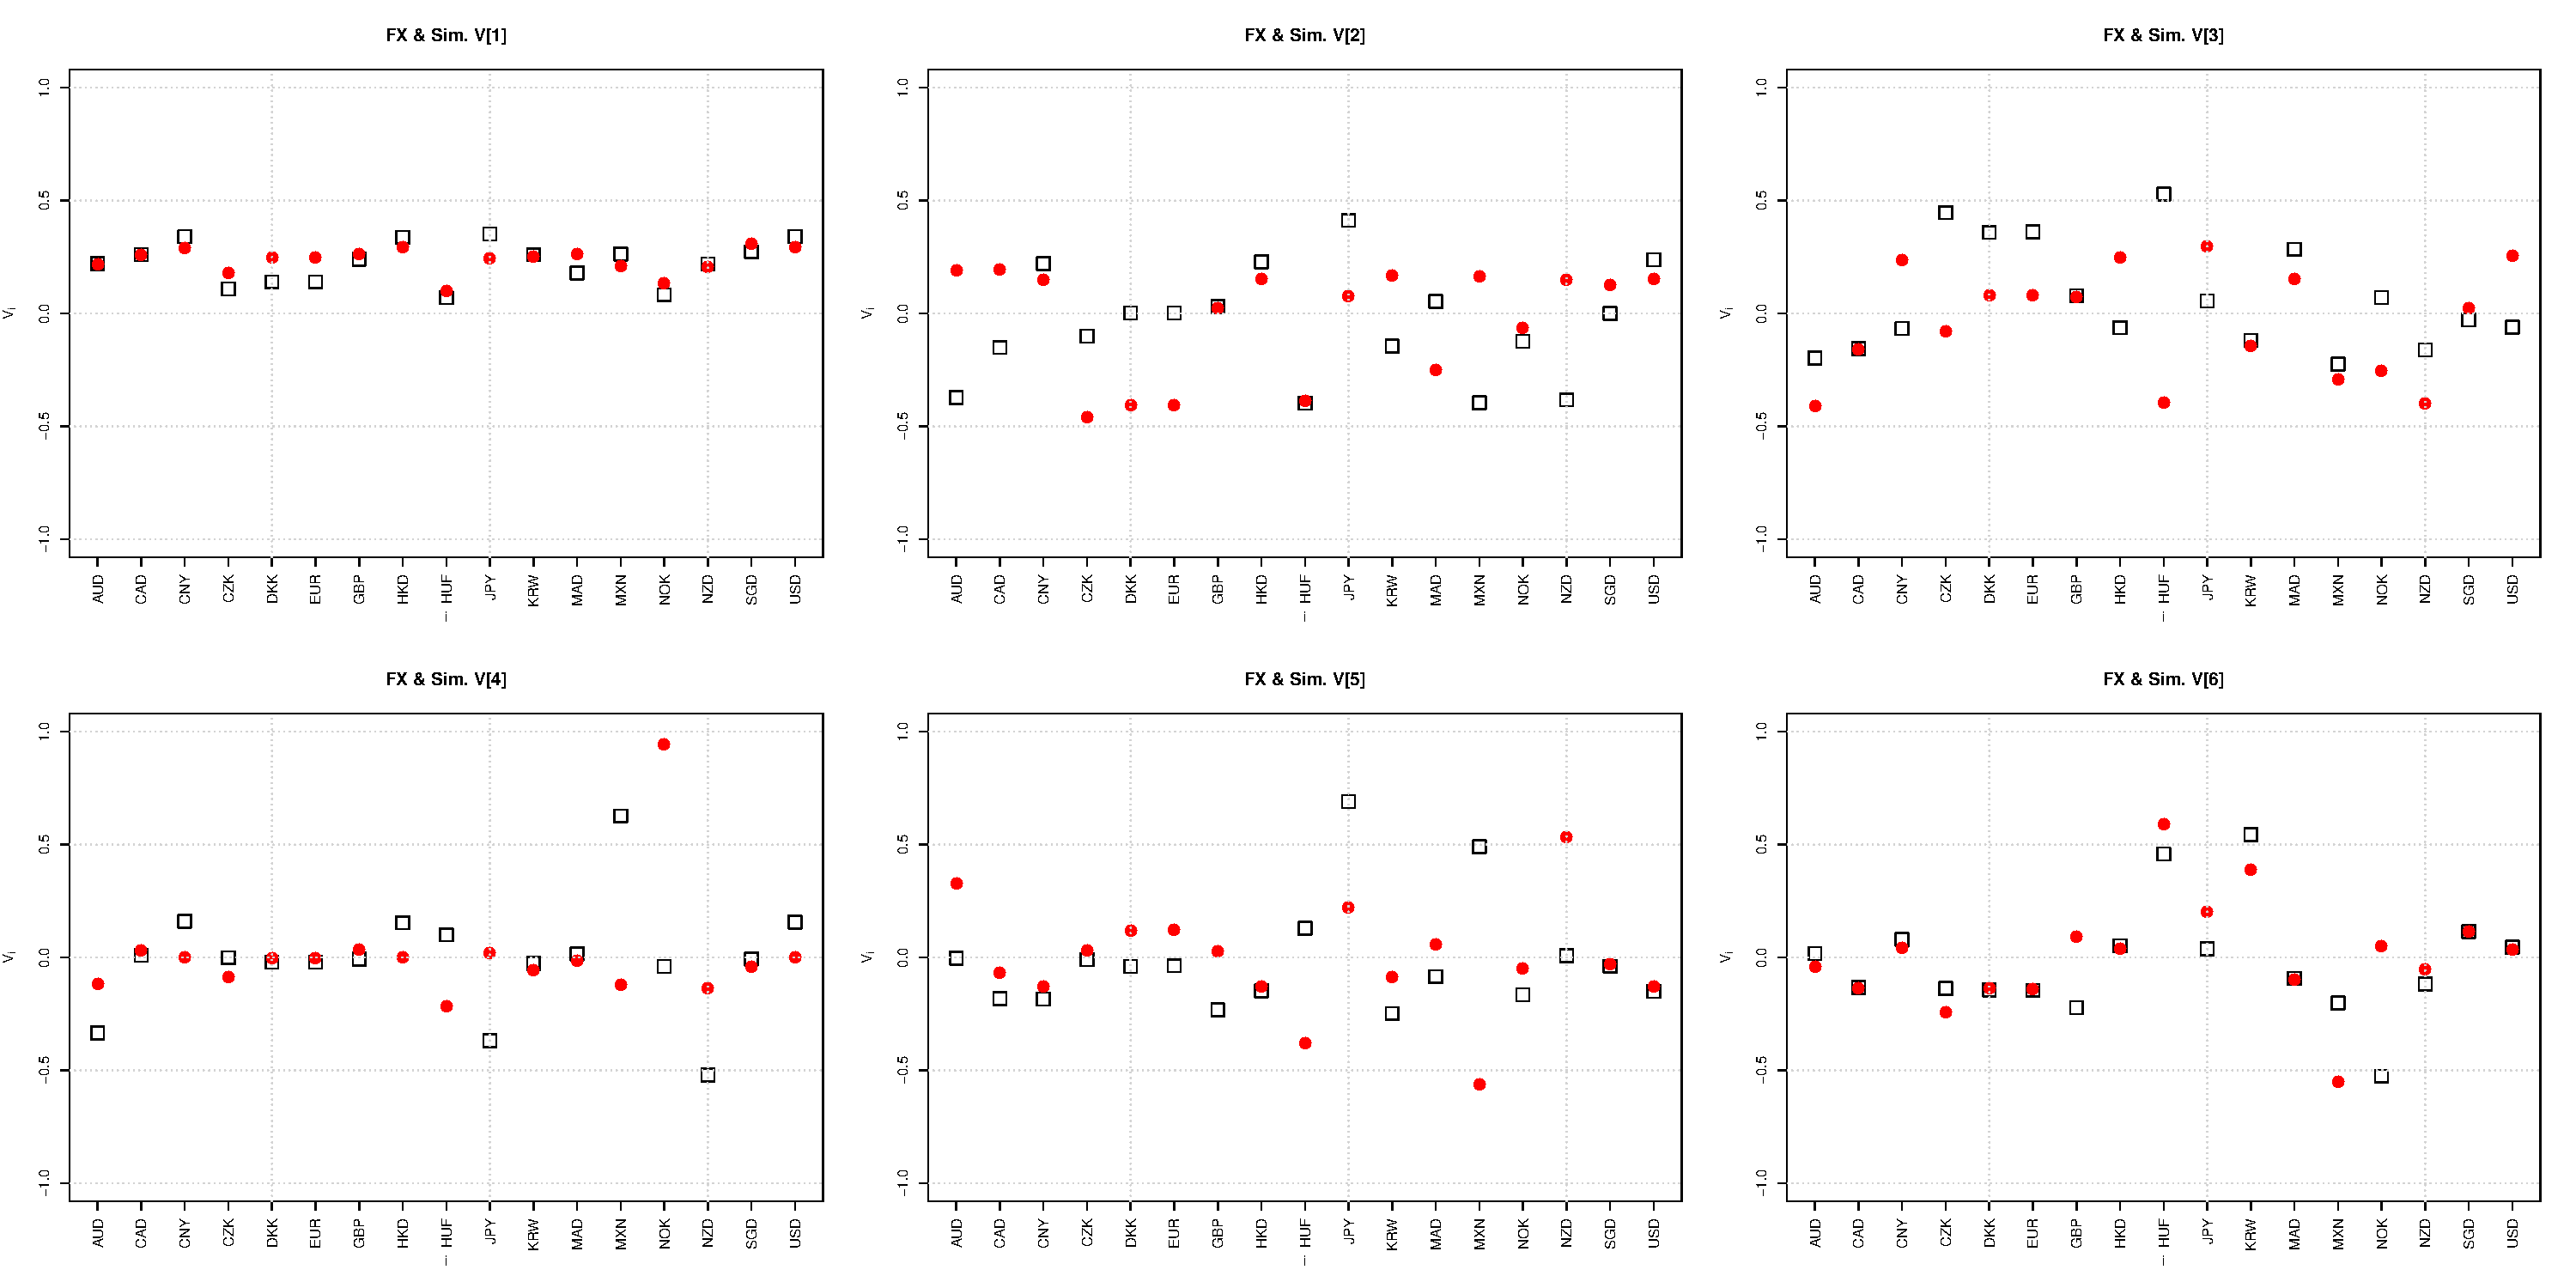
\includegraphics[scale=0.2]{Gaussian_eigenvectors.pdf}
    \caption{\scriptsize Eigenvectors of real FX series and Simulated Gaussian series}
  \end{figure}
\end{frame}

\begin{frame}
  \frametitle{Emergence of the Observed Spectrum}
  Joint regular variation of the entries of the covariance matrix can
  produce delocalized eigenvectors as seen in the data:
  \[
  \lim_{u \to \infty} u^{\kappa}
  \P\left(
    \inn{\vec{x}, V} > u
  \right) = e_{\kappa}(\vec{x}),\; \vec x \in \mathbb S^{p-1}
  \]
  where $V=(\E X_{1,t}^2, ..., \E X_{p,t}^2,
  \{\E (X_{i,t}X_{j,t})\}_{1 \leq i < j \leq p})$

  This way, we have a covariance matrix where some of the non-diagonal
  entries are non-zero under proper normalization.
\end{frame}

\begin{frame}
  \frametitle{The Tail index $\kappa_i$}
  Consider the tail indices of the entries of the covariance matrix C:
  For the diagonal entries
    \begin{eqnarray*}
      C_{i, i} &=& a_n^{-1} \sum_{t=1}^n X_{i, t}^2 \\
      &=& a_n^{-1} \sum_{t=1}^n Z_{i, t}^2 \sigma_{i, t}^2 \\
    \end{eqnarray*}
    $Z_{i, t}^2$ is light tailed, so $Z_{i, t}^2 \sigma_{i, t}^2$ has
    the same tail index as $\sigma_{i, t}^2$, which is given by
    \[
    \E (\alpha_i Z^2 + \beta_i)^{\kappa_i} = 1
    \]
    where $Z \sim N(0, 1)$.
  \end{frame}

  \begin{frame}
  \frametitle{The Tail index $\kappa_{i,j}$}
    For the non-diagonal entries
    \begin{eqnarray*}
      C_{i, j} &=& b_n^{-1} \sum_{t=1}^n X_{i, t} X_{j, t} \\
      &=& b_n^{-1} \sum_{t=1}^n Z_{i, t} Z_{j, t} \sigma_{i, t} \sigma_{j, t}
    \end{eqnarray*}
    Again, $Z_{i, t} Z_{j, t} \sigma_{i, t} \sigma_{j, t}$ has the
    same tail index as $\sigma_{i, t} \sigma_{j, t}$, which is given
    by
    \[
    \E [(\alpha_i Z_i + \beta_i)^{\kappa_{i,j}}(\alpha_i Z_i +
    \beta_i)^{\kappa_{i,j}}] = 1
    \]
  \end{frame}


  % \begin{itemize}
  % \item For a GARCH(1,1) process
  %   \[
  %   \E (\alpha Z^2 + \beta)^\kappa = 1
  %   \]
  %   gives the index of regular variation $\kappa$ of $\sigma_{i, t}^2$.
  % \item For $\E (X_{i,t} X_{j,t})$:
  %   \begin{eqnarray*}
  %     && \E (X_{i,t} X_{j,t})      \\
  %     &=& \E (Z_{i,t} Z_{j, t}) \E (\sigma_{i,t} \sigma_{j, t})
  %   \end{eqnarray*}
  % \end{itemize}



\subsection{IARCH(1), ARCH(1) and IGARCH(1) processes}
\begin{frame}
  \frametitle{IARCH(1)}
  In the special case of IARCH(1), i.e. $\alpha_{i} = 1$, $\beta_{i,
    1} = 0$,
  \[
  \E (Z_i^2)^{\kappa_i} = 1
  \]
  gives $\kappa_i = 1$. Suppose
  \begin{eqnarray*}
    \E (Z_i^2 Z_j^2)^\kappa &=& 1 \\
    (Z_i, Z_j) &\sim& N(0, \Sigma) \\
    \Sigma &=&
    \begin{pmatrix}
      1 & \rho \\
      \rho & 1
    \end{pmatrix}
  \end{eqnarray*}
  $\E (Z_i^2 Z_j^2)^\kappa = 1$ means
  \begin{eqnarray*}
    && {1 \over 2\pi}
    \int \int
    \left(
      \rho^2 x^4 + (1 - \rho^2) x^2 y^2 + 2 \rho \sqrt{1 - \rho^2} x^3 y
    \right)^\kappa \times \\
    &&
    \exp\left(
      -{x^2 + y^2 \over 2}
    \right)
    dx dy = 1
  \end{eqnarray*}
  When $\rho = \pm 1$, it is clear $\kappa = 1/2$.  
\end{frame}

\begin{frame}
  \frametitle{IARCH(1)}
  When $-1 < \rho < 1$, re-writing in polar coordinates gives
  \begin{eqnarray*}
    && {1 \over 2\pi} \int_0^{\infty} r^{4\kappa + 1} e^{-r^2 / 2} dr
    \int_{0}^{2\pi} \cos(\theta)^{2 \kappa} \times \\
    &&
    \left(
      2 \rho^2 \cos(\theta)^2
      + 2 \rho \sqrt{1 - \rho^2} \cos(\theta) \sin(\theta) - \cos(\theta)^2 + 1 - \rho^2
    \right)^\kappa d\theta = 1
  \end{eqnarray*}
  Inegrating the radial part gives
  \begin{eqnarray*}
    && \int_{0}^{2\pi}
    \cos(\theta)^{2\kappa}
    \left(
      2 \rho^2 \cos(\theta)^2 + \rho \sqrt{1 - \rho^2} \sin(2\theta) - \cos(\theta)^2 - \rho^2 + 1
    \right)^\kappa \times \\
    && d\theta
    = {2 \pi
      \over
      2^{2 \kappa} \Gamma(2\kappa + 1)
    }
  \end{eqnarray*}
\end{frame}

\begin{frame}
  \frametitle{IARCH(1)}
  After some manipulations we arrive at
  \begin{equation}
    \int_{-1}^1 (\sin(\pi z) + \rho)^{2\kappa} dz = {2 \over \Gamma(2\kappa + 1)}
  \end{equation}
  Using this result, we immediately obtain for ARCH(1) models
  \begin{equation*}
    \int_{-1}^1 (\sin(\pi z) + \rho)^{2\kappa} dz =
    {2 \over \Gamma(2\kappa + 1)}
    {1 \over (\alpha_{i} \alpha_{j})^\kappa}
  \end{equation*}
  So Non-diagonal entries of the empirical covariance matrix can have
  a tail as heavy as the heaviest of the diagonal entries.
\end{frame}

\begin{frame}
  \frametitle{ARCH(1)}  
  ARCH(1) models fit the data too.
  \begin{figure}[htb!]
    \centering
    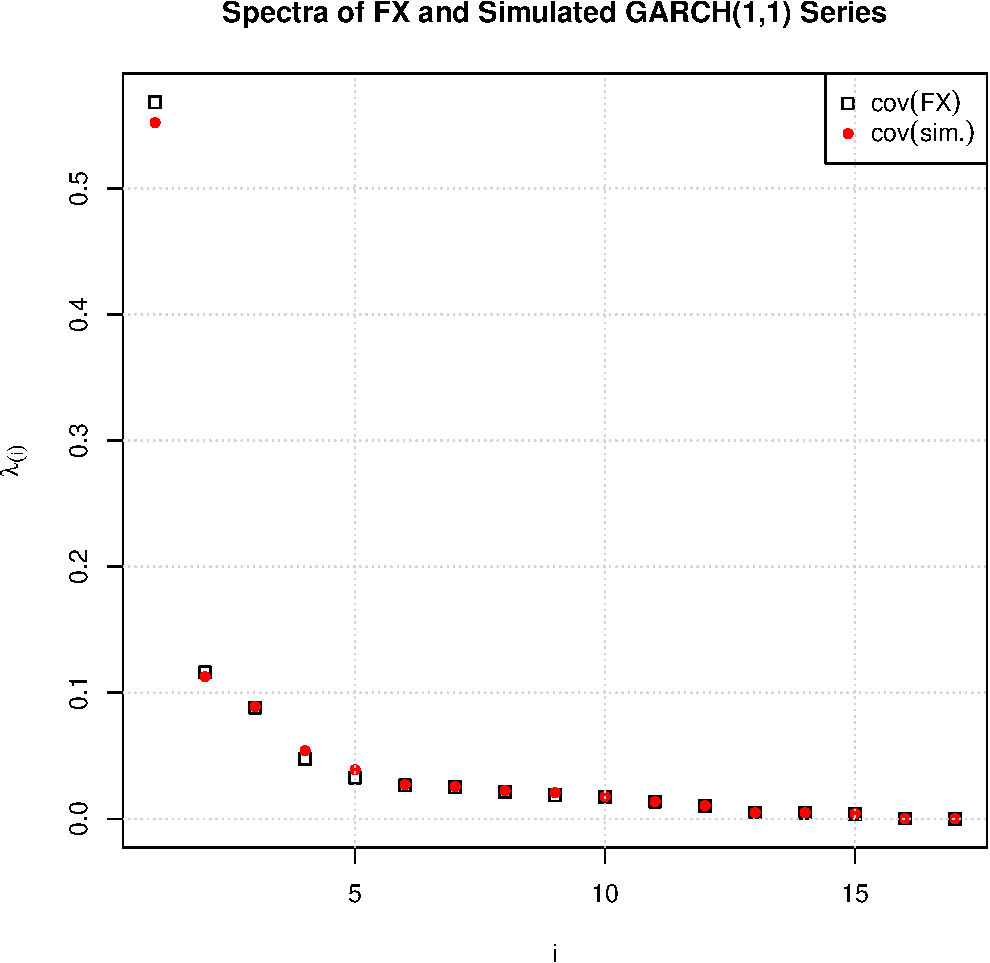
\includegraphics[scale=0.35]{FX_eigenvalues.pdf}  
    \caption{FX \& simulated ARCH eigenvalues}
    \label{fig:FX_ARCH_eigenvalues}
  \end{figure}
\end{frame}

\begin{frame}
  \begin{figure}[htb!]
    \centering
    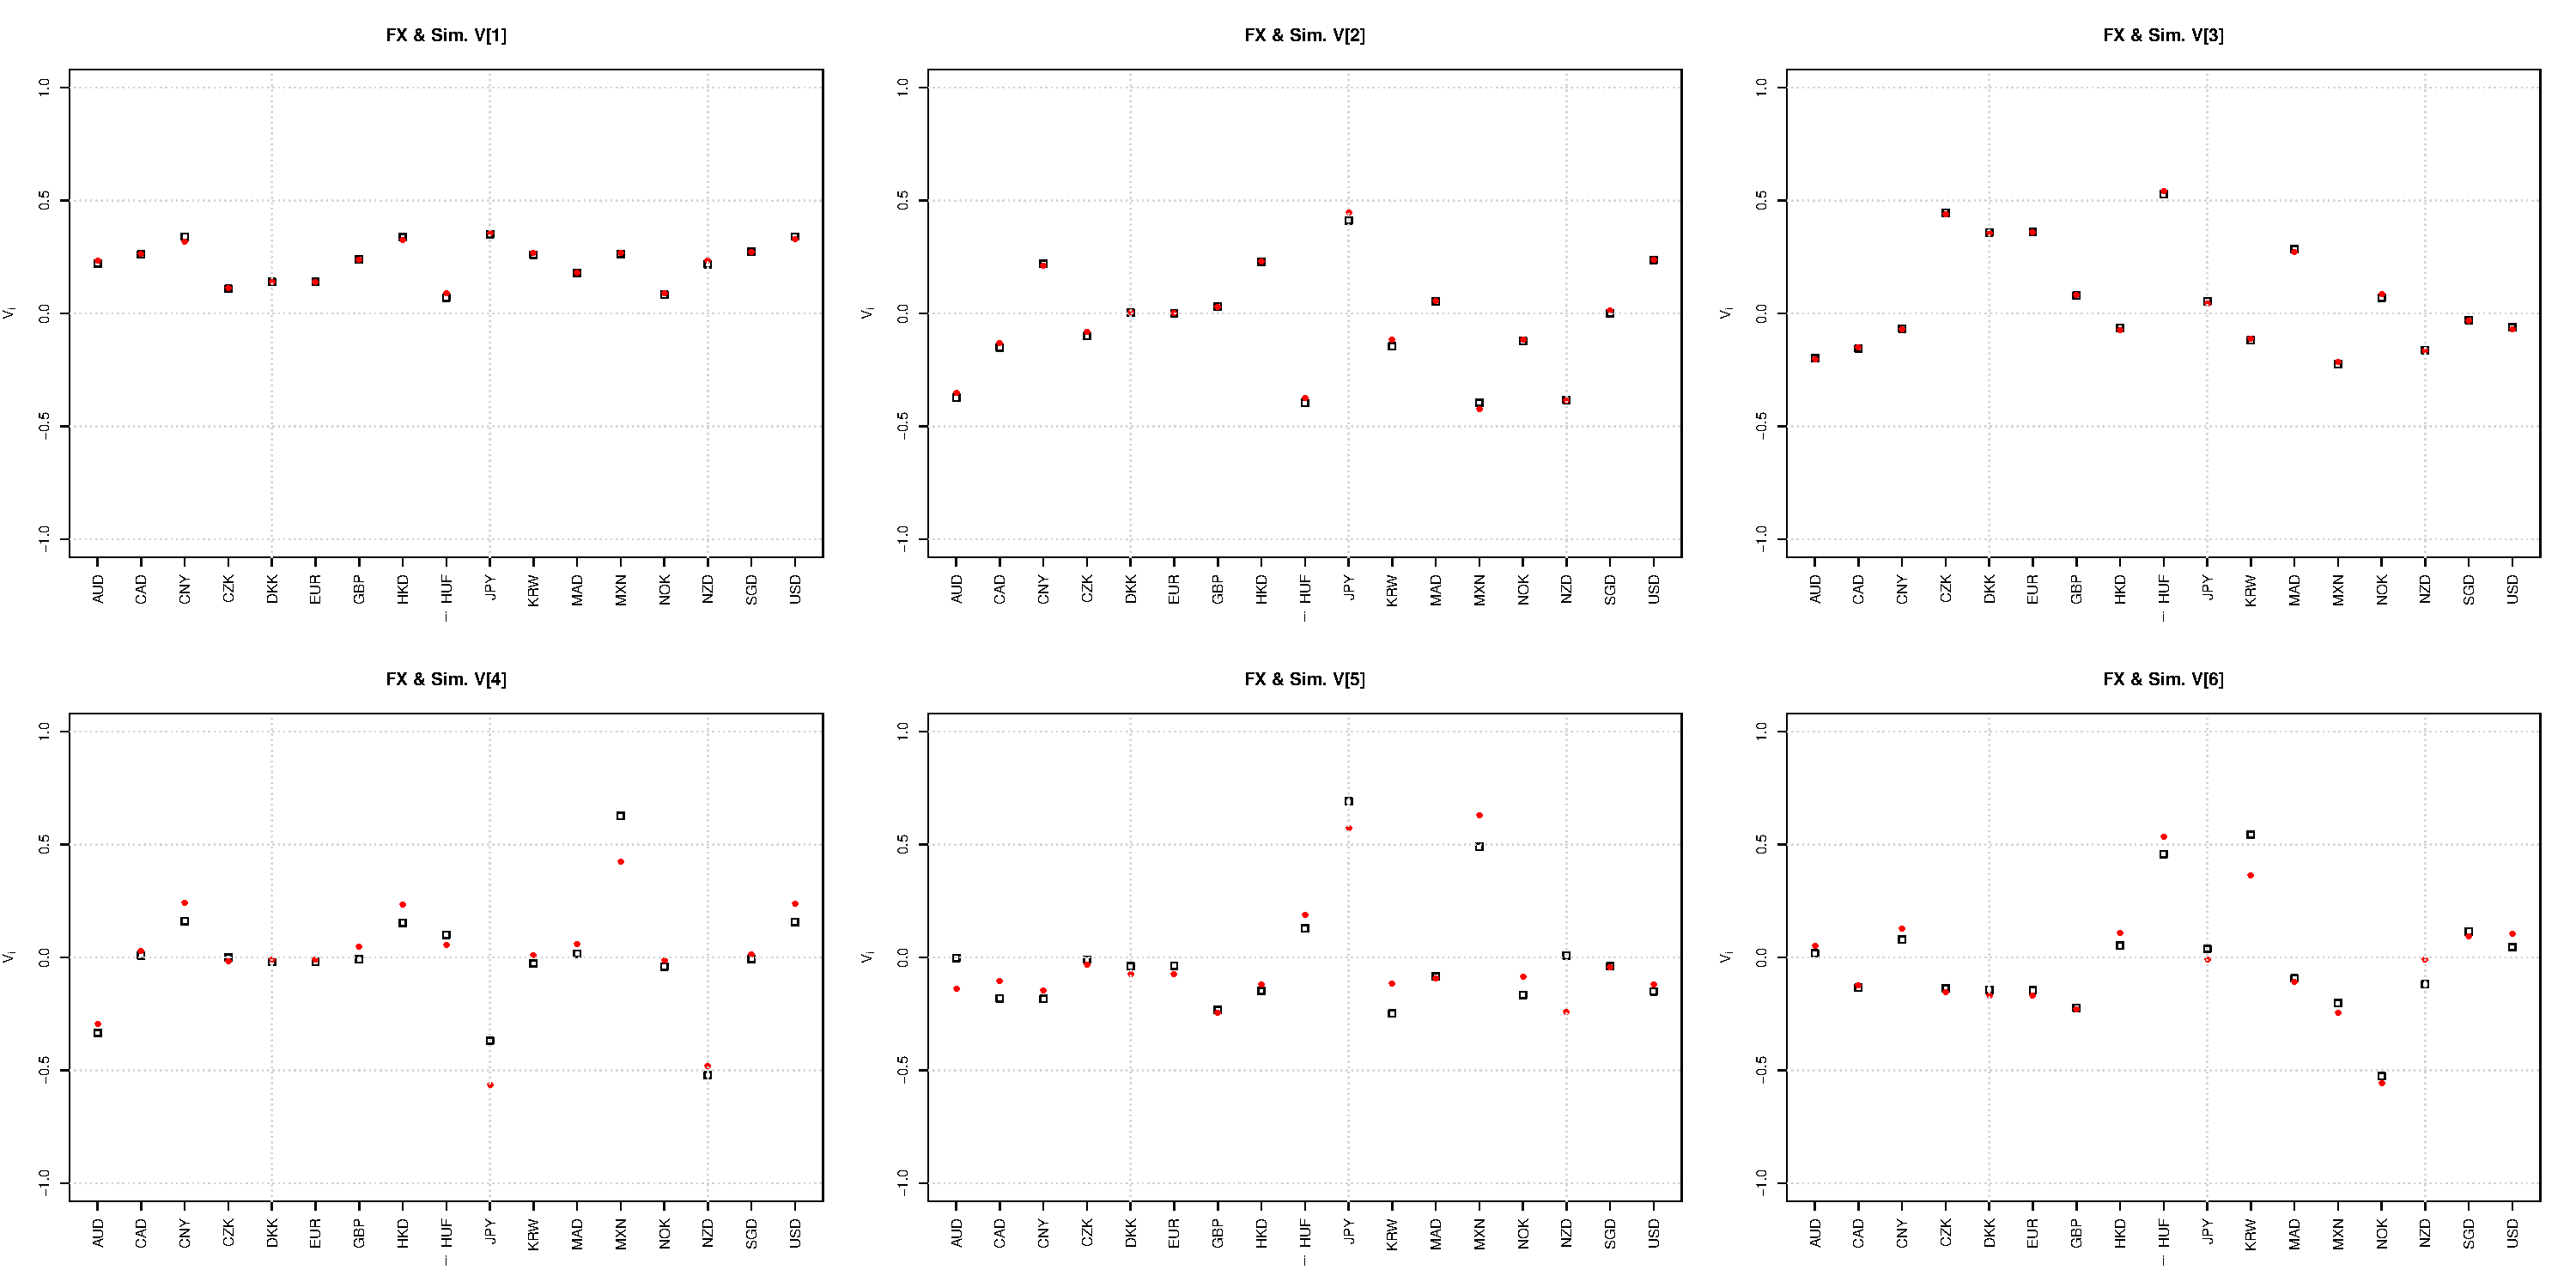
\includegraphics[scale=0.1]{FX_eigenvectors.pdf}  
    \caption{FX \& ARCH eigenvectors}
    \label{fig:FX_ARCH_eigenvectors}
  \end{figure}
\end{frame}
\bibliographystyle{unsrt}
\bibliography{../../thesis/econophysics}
\end{document} 

